\documentclass[12pt, letterpaper]{article}
\usepackage[OT4]{fontenc}
\usepackage[polish]{babel}
\usepackage{graphicx}
\usepackage{url}
\usepackage{hyperref}
\graphicspath{{images/}}

\hypersetup{
 colorlinks=true,
 citecolor=,
 linkcolor=,
 urlcolor=}

\title{\textbf{Finał UCL 2023}}
\author{Rafał Mielniczuk}
\date{\today}

\begin{document}

\maketitle

\tableofcontents
\pagebreak


\section{Problem badawczy}
\paragraph{} W piłce nożnej wszystko jest możliwe. Nawet słabsza drużyna zawsze ma realne szanse na wygraną meczu, chociaż jego wynik sugerowałby zupełnie co innego. Zgodnie z tą myślą finał UEFA Champions League (UCL) może przynieść zaskakujące rezultaty. Co więcej, wyniki półfinałów mogłby być już dla niektórych zaskoczeniem. \par Przedstawia to oczywisty problem: czy można na podstawie dostępnych danych z obecnych sezonów ligowych i zeszłych rozgrywek UCL wyłonić zasłużonych finalistów oraz zwycięzcę tegorocznego UCL. Ze względu na rozważanie finału problem jest ograniczony tylko do tegorocznych półfinalistów - AC Milan, Internazionale Mediolan, Real Madrid, Manchester City.


\section{Dane}
\subsection{Pozyskane dane}
\subsubsection{Zakres}
\paragraph{} Najważniejszym czynnikiem pozwalającym na ocenę szans danej drużyny jest jej obecna forma, dlatego należy uwzględnić w pozyskanych danych obecny sezon. Ponadto drużyny nie zawsze przywiązują taką samą wagę do rozgrywek domowych, co do rozgrywek europejskich. Z tego powodu należy również zawrzeć w danych informacje o poprzednich rozgrywkach UCL. Ze względu na dynamikę piłki nożnej i częste rotacje w składach drużyn tylko dane z ostatnich 5 lat zostaną uwzględnione. Ponadto będą to dane tylko rozgrywek 1/8 bądż wyżej, ponieważ odpadnięcie w grupie dla drużyn na tym poziomie jest nieudanym sezonem.
\subsubsection{Szczegóły}
\paragraph{} Do zakresu analizowanych danych należą statystyki strzałów oraz piłkarzy drużyn w meczu. Przykładowo: \pagebreak
\begin{figure}[ht]
    \centering
    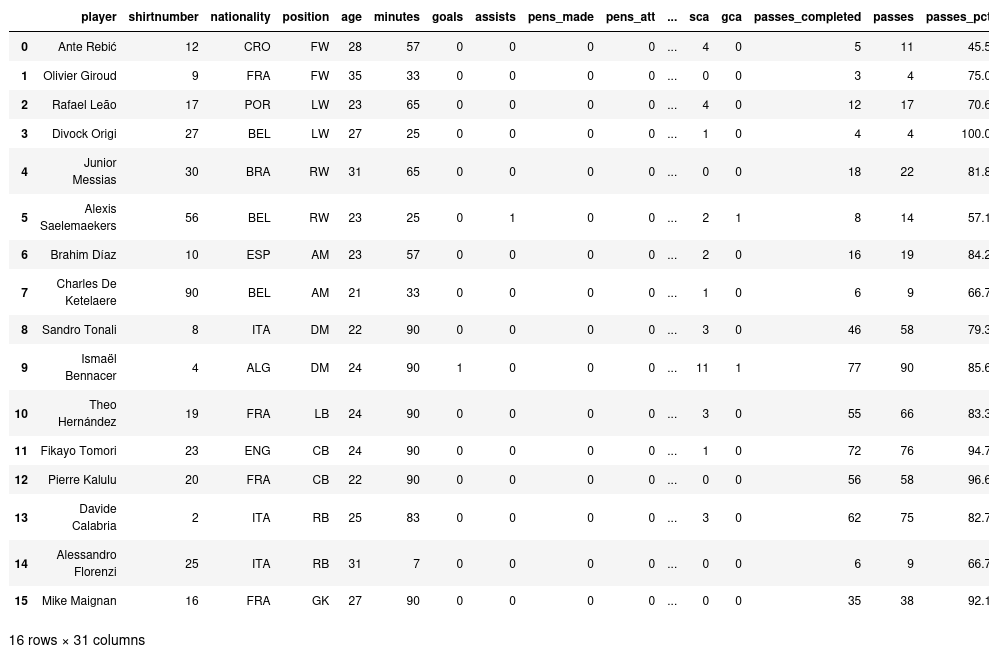
\includegraphics[width=0.67\textwidth]{images/example_players.png}
\end{figure}
\begin{figure}[ht]
    \centering
    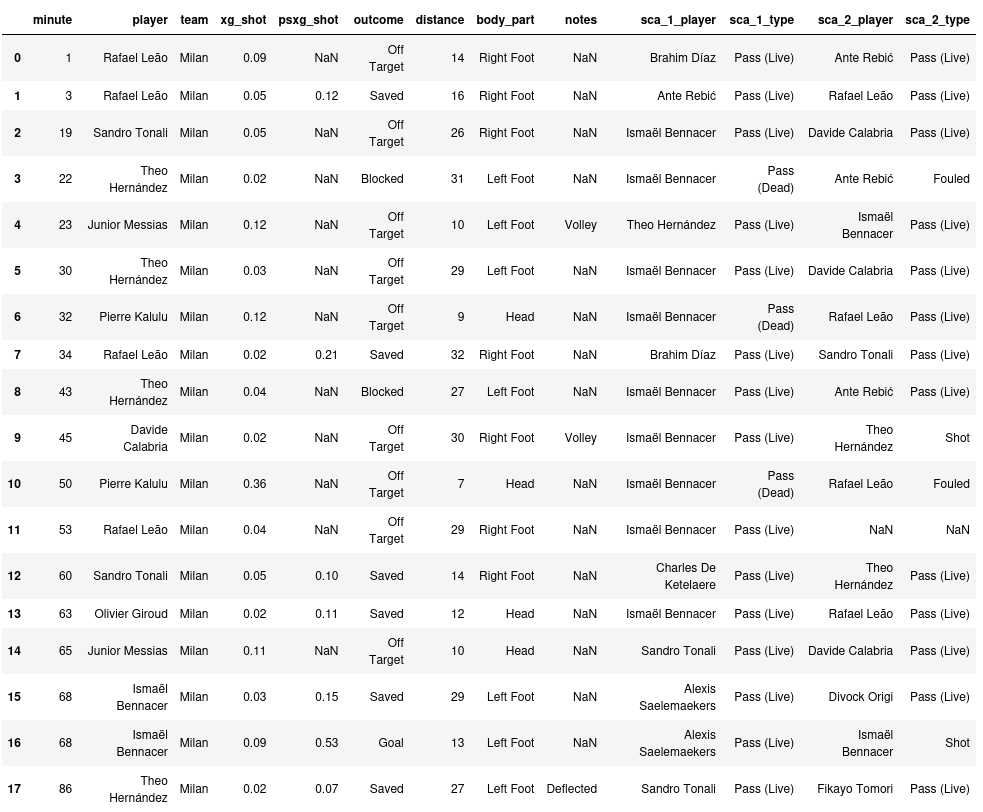
\includegraphics[width=0.67\textwidth]{images/example_shots.png}
\end{figure}
\paragraph{} W danych piłkarzy można wyróżnić kolejno: imię i nazwisko, numer koszulki, pozycja, wiek, rozegrane minuty, gole, asysty, rzuty karne wykonane, próby rzutów karnych, ilość strzałów, ilość strzałów na bramkę, żółte kartki, czerwone kartki, kontakty, przejęcia, przechwycenia, bloki, oczekiwane gole, oczekiwane gole bez rzutów karnych, oczekiwane gole po asyście, liczba akcji kreujących strzał, liczba akcji kreujących gol, udane podania, podania, skuteczność podań, progresywne podania, kontrola piłki, progresywna kontrola piłki, dryblingi, udane dryblingi.
\paragraph{} W danych strzałów można wyróżnić kolejno: minuta, imię i nazwisko, klub, oczekiwane gole, oczekiwane gole uwzględniając pozycję bramkarza, rezultat, dystans do bramki, część ciała, adnotacje, gracze i wydarzenia kreujące akcję.
\subsubsection{Sposób}
\paragraph{} Dane zostały pozyskane poprzez web scraping\cite{link}.
\subsection{Odrzucone dane}
\subsubsection{Zakres}
\paragraph{} Analizując występy drużyn należy skupiać się również na poszczególnych jednostkach, które się na nią składają. Nie zawsze jednak można porównać dwóch zawodników. Niektórzy z nich pojawiają się na murawie tylko w celach strategicznych, aby skrócić rozgrywany czas trwania meczu. Wchodzą w ostatnich minutach meczu i ich występ statystycznie wypada bardzo słabo na tle innych zawodników. Ponadto bramkarze mają specyficzną rolę, która jest ciężka do porównania do innych zawodników w polu. \par Z wyżej wymienionych powodów statystyki zawodników będących na murawie ponieżej 10 minut i bramkarzy nie będą brane pod uwagę.
\subsubsection{Szczegóły}
\paragraph{} Ponieważ szczegółowość dostarczonych danych jest zbyt duża na potrzeby rozważanego raportu, dane zostaną ograniczone. \par Dane graczy kolejno: imię i nazwisko, pozycja, rozegrane minuty, gole, asysty, oczekiwane gole, oczekiwane gole po asyście, liczba akcji kreujących strzał, liczba akcji kreujących gol, udane podania, podania, skuteczność podań. \par Dane strzałów kolejno: minuta, imię i nazwisko, klub, oczekiwane gole, rezultat.


\section{Analiza danych}
\subsection{Rozgrywki ligowe}
\paragraph{} Każda z analizowanych drużyn rozegrała w tym sezonie 38 spotkań w rozgrywkach domowych. Do analizy zostaną poddane najważniejsze statystyki pozwalające zwyciężać, czyli okazje strzeleckie, szanse na zdobywanie bramek oraz dokładność podań drużyny. Zwycięstwa nie mają aż tak dużego znaczenia, ponieważ piłka nożna jest nieprzewidywalna. Natomiast stałe dobre rezultaty pozwalają zobaczyć, czy drużyna rzeczywiście reprezentowała wysoką formę. Szczególną uwagę można zwrócić na okres fazy pucharowej ligi mistrzów zaczynający się mniej więcej w trakcie kolejki 22.

\subsubsection{AC Milan}
\begin{figure}[ht]
    \centering
    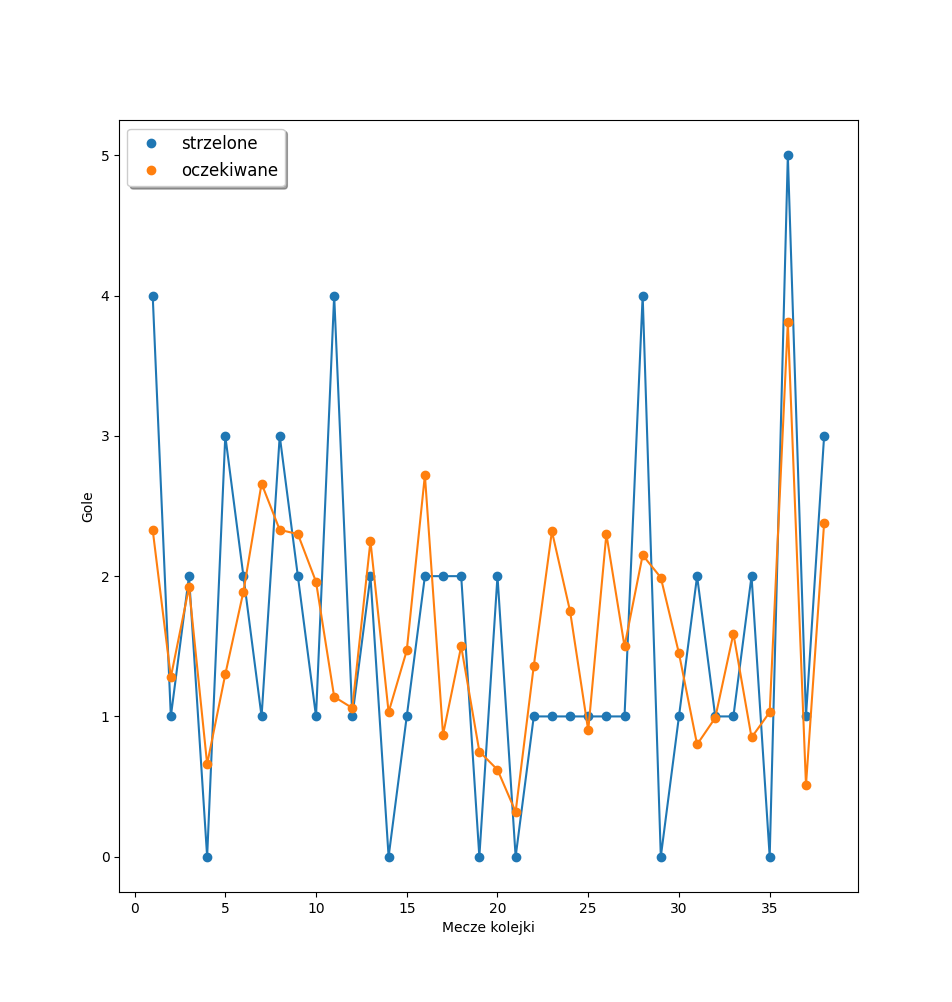
\includegraphics[width=.8\textwidth]{images/Milan_goals.png}
    \caption{Gole AC Milanu}
    \label{fig:enter-label}
\end{figure}
\paragraph{} W przypadku goli można zauważyć stałą tendencję do 1 lub 2 bramek na mecz. Można uznać AC Milan pod tym względem za dość stabilną drużynę.
\pagebreak
\begin{figure}[ht]
    \centering
    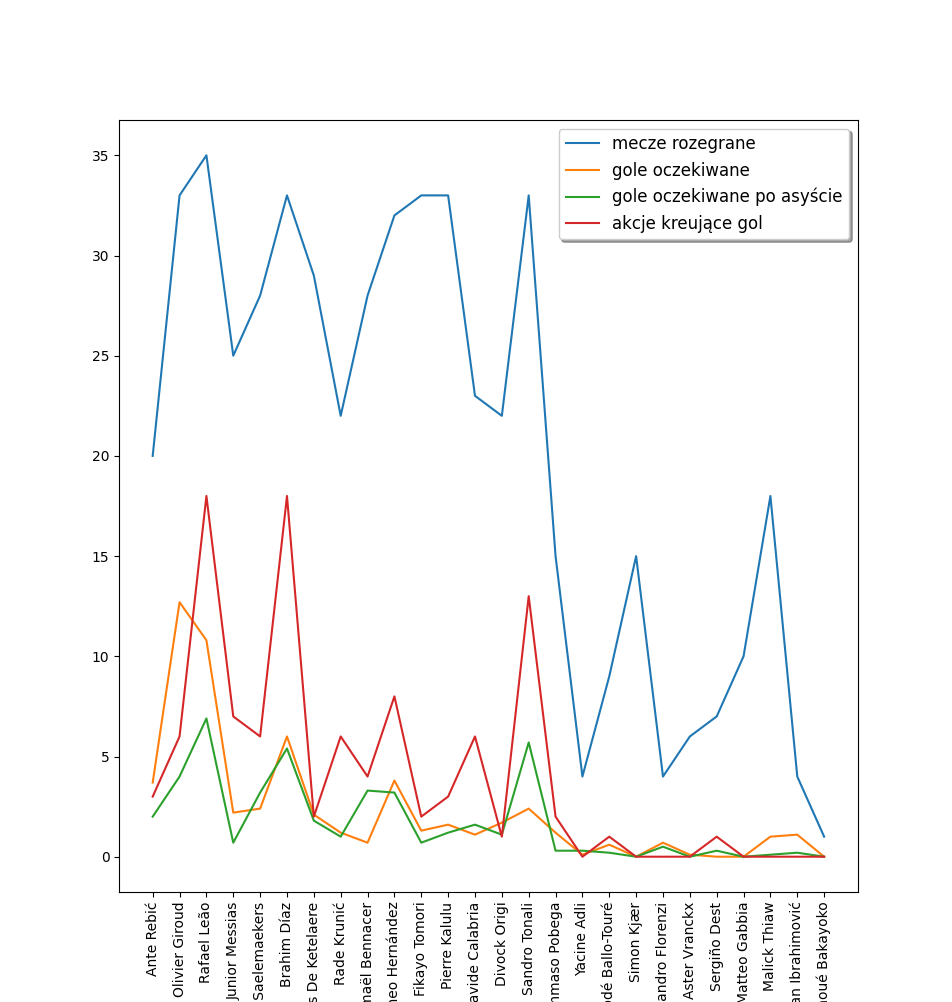
\includegraphics[width=0.8\textwidth]{images/Milan_player_goals.png}
    \caption{Gole graczy AC Milanu}
    \label{fig:enter-label}
\end{figure}
\paragraph{} Można zauważyć, że analizowany zespół opiera swoją grę głównie na kilku zawodnikach, gdzie przeważnie Oliver Giroud i Rafael Leao mają okazje strzeleckie, natomiast akcje wyprowadzane są głównie przez S.Tonalego, B.Diaza oraz ponownie R.Leao.
\pagebreak
\begin{figure}[ht]
    \centering
    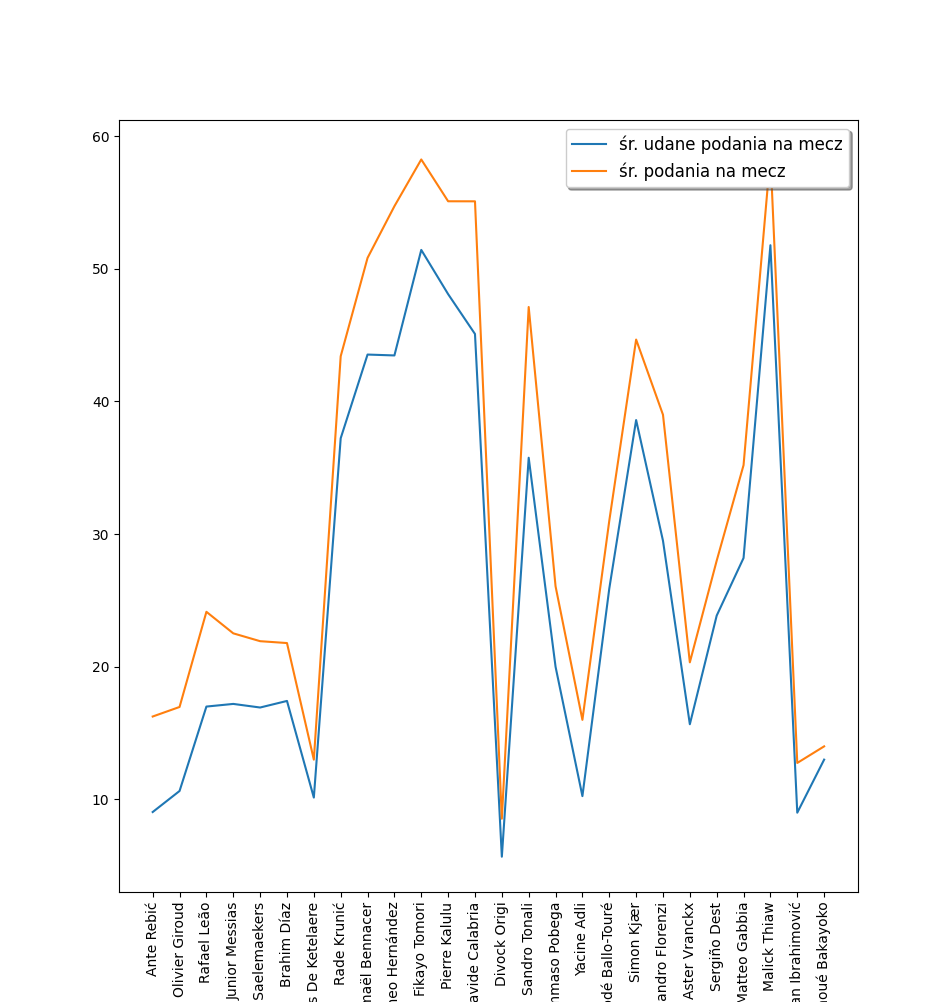
\includegraphics[width=0.8\textwidth]{images/Milan_passes.png}
    \caption{Podania graczy AC Milanu}
    \label{fig:enter-label}
\end{figure}
\paragraph{} Drużyna bardzo słabo wypada na europejskim poziomie w kwestii podań i ich dokładności. U wielu zawodników można zauważyć dużą, jak na reprezentowany przez nich poziom, różnicę między udanymi, a wykonanymi podaniami. Ponadto liczba podań jest przeważnie mała. Sugeruje to długie piłki i grę z kontry.
\pagebreak

\subsubsection{Internazionale Mediolan}
\begin{figure}[ht]
    \centering
    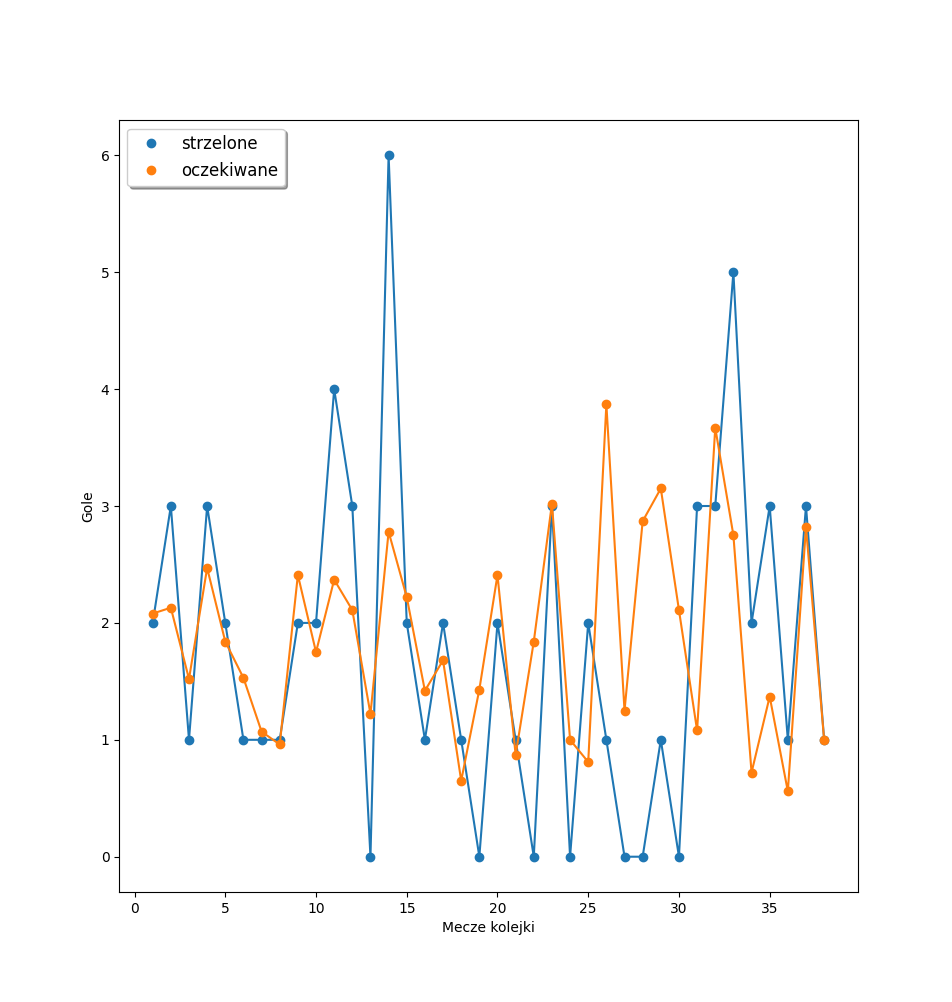
\includegraphics[width=.8\textwidth]{images/Inter_goals.png}
    \caption{Gole Internazionale Mediolan}
    \label{fig:enter-label}
\end{figure}
\paragraph{} Gole na mecz Internazionale Mediolan, zwanego również potoczine Nerazzurri bądź Inter, również oscylują w przedziale od 1 do 2. Nawet można zauważyć wzrost goli oczekiwanych pod koniec sezonu, to jest w okresie trwających rozgrywek UCL.
\pagebreak
\begin{figure}[ht]
    \centering
    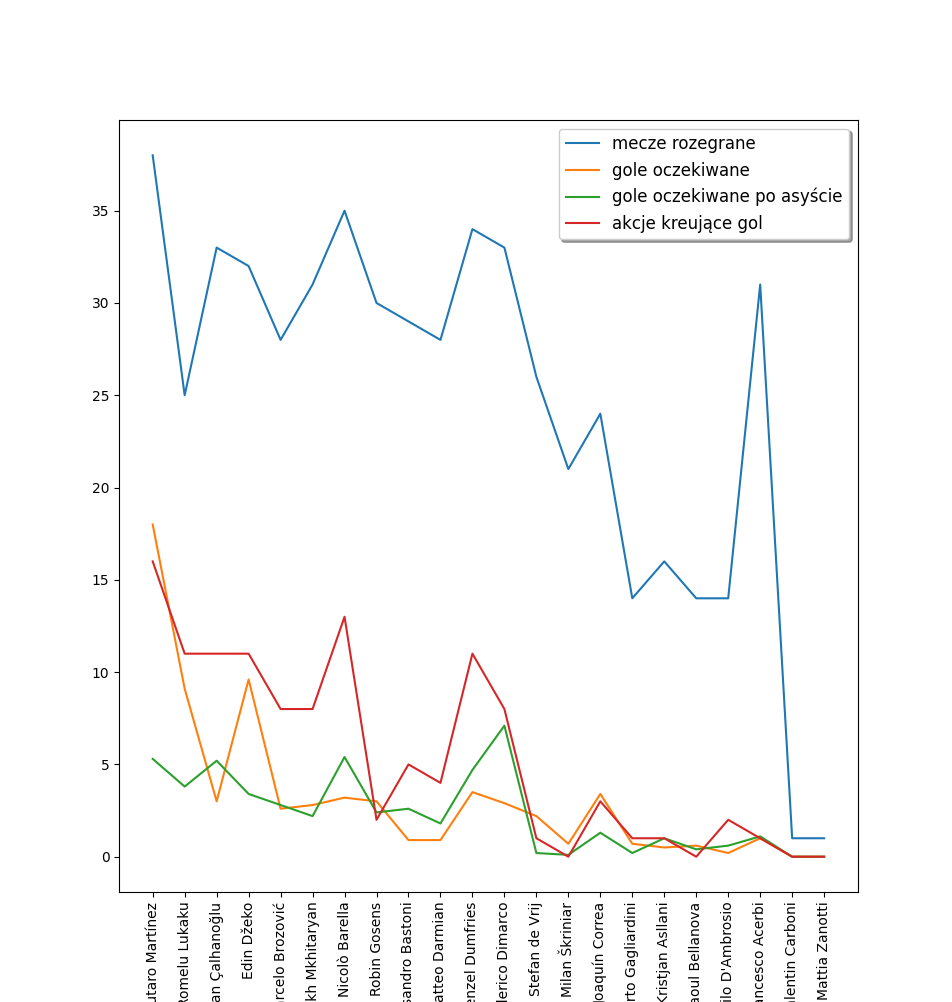
\includegraphics[width=0.8\textwidth]{images/Inter_player_goals.png}
    \caption{Gole graczy Internazionale Medional}
    \label{fig:enter-label}
\end{figure}
\paragraph{} Nerazzurri ma dużo solidnych graczy wyprowadzających akcje. Ich gra może się wydawać bardziej rozłożona i niezależna od kilku jednostek. Natomiast gole są strzelane przeważnie przez ich napastników - R.Lukaku, L.Martineza i E.Dzeko. Godny wyróżnienia jest również F.Dimarco, którego podania stwarzają duże zagrożenie bramkowe.
\pagebreak
\begin{figure}[ht]
    \centering
    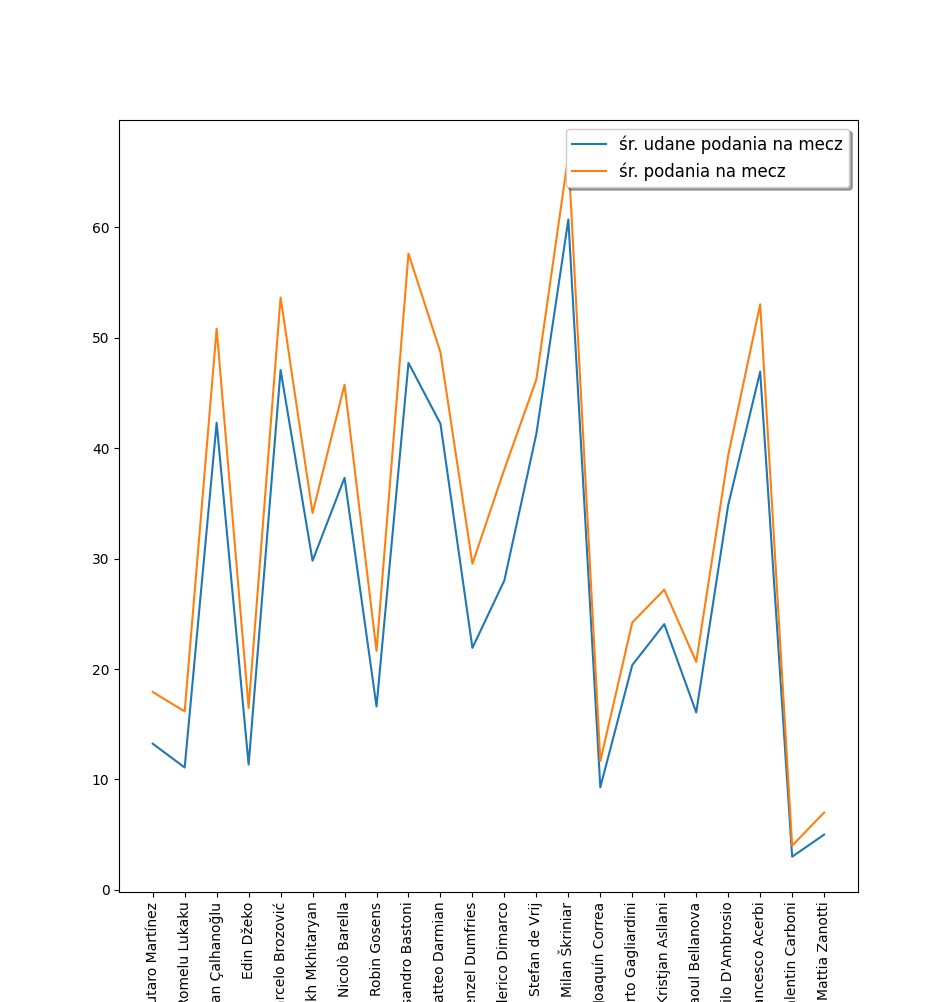
\includegraphics[width=0.8\textwidth]{images/Inter_passes.png}
    \caption{Podania graczy Internazionale Mediolan}
    \label{fig:enter-label}
\end{figure}
\paragraph{} Podania zawodników Interu cechują się przeważnie w dużą dokładnością. Ponadto ich średnia jest stosunkowo dużo, co może świadczyć o defensywnej grze lub wolno budowanych akcjach.
\pagebreak

\subsubsection{Real Madrid}
\begin{figure}[ht]
    \centering
    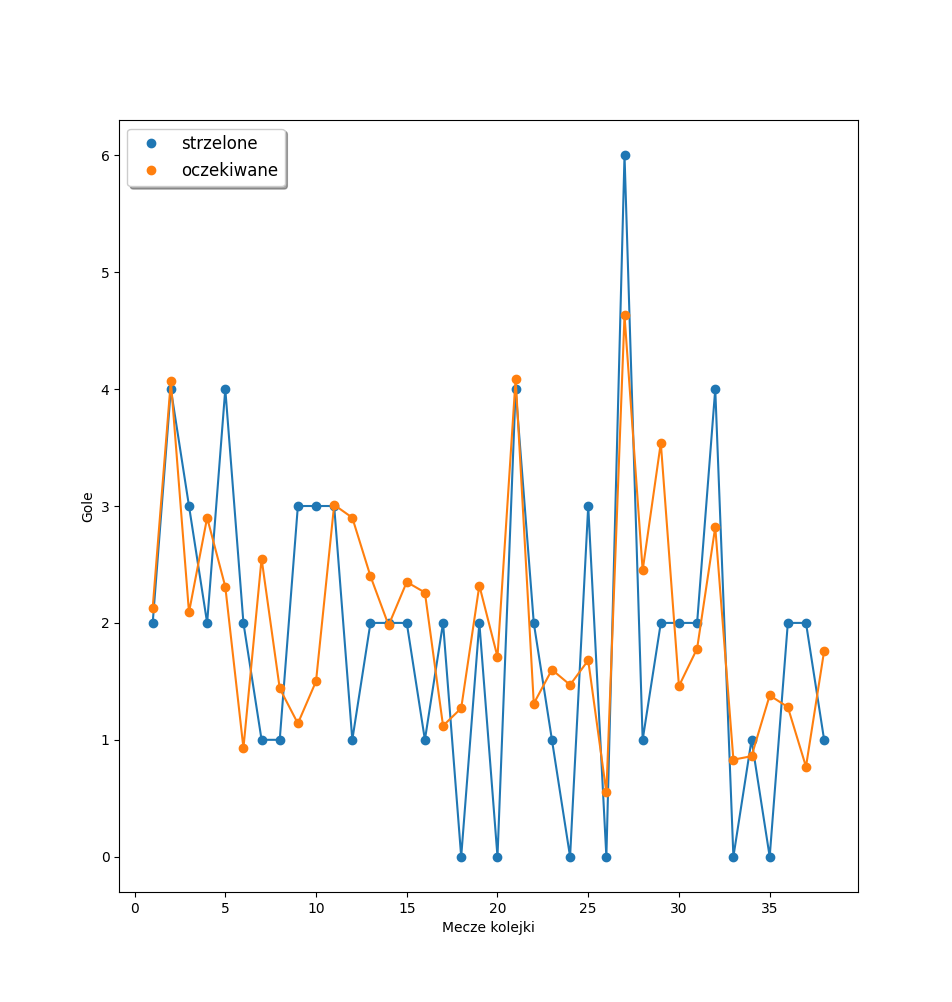
\includegraphics[width=.8\textwidth]{images/Real_goals.png}
    \caption{Gole Realu Madrid}
    \label{fig:enter-label}
\end{figure}
\paragraph{} Real ma dość wysoką średnią goli w okolicach 2. Ponadto ich oczekiwane gole często sięgają aż 3.
\pagebreak
\begin{figure}[ht]
    \centering
    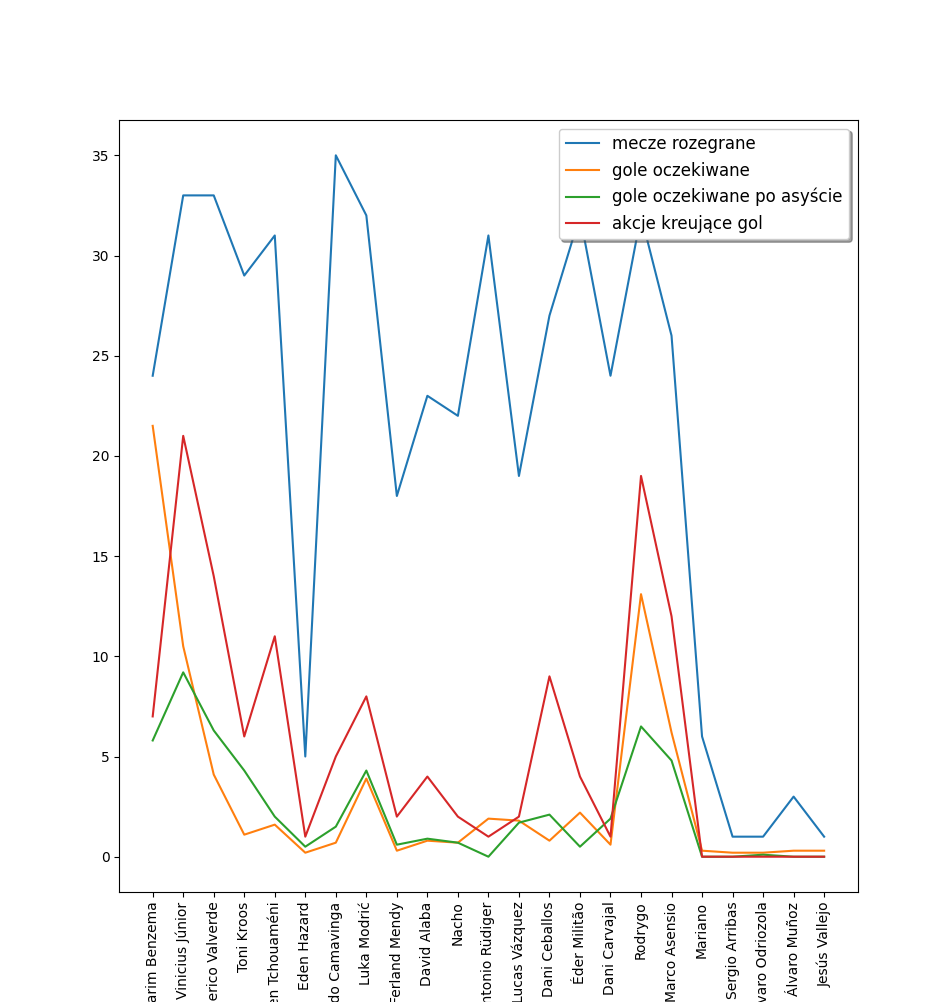
\includegraphics[width=0.8\textwidth]{images/Real_players_goals.png}
    \caption{Gole graczy Realu Madrid}
    \label{fig:enter-label}
\end{figure}
\paragraph{} Z wykresu można zauważyć, że drużyna ma nadzwyczaj uniwersalną drużynę, gdzie dużo osób jest w stanie kreaować akcje bramkowe i wykonywać podania z dużą szansą na bramkę. Jednak da się zauważyć trzech głównych strzelców, czyli K.Benzemę, Viniciusa oraz Rodrygo.
\pagebreak
\begin{figure}[ht]
    \centering
    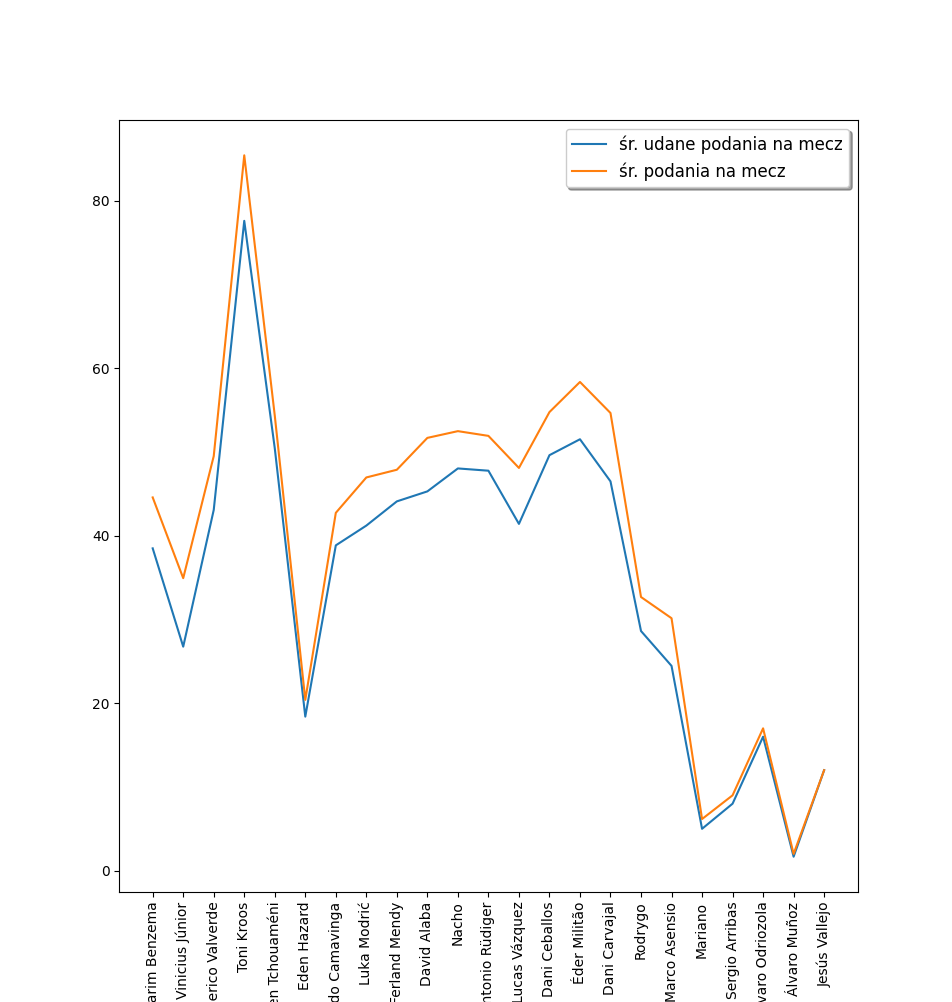
\includegraphics[width=0.8\textwidth]{images/Real_passes.png}
    \caption{Podania graczy Realu}
    \label{fig:enter-label}
\end{figure}
\paragraph{} Podania graczy analizowanego zespołu są równomiernie rozłożone, co sugeruje, że grają równo na szerokości całego boiska. Zwłaszcza duża ilość podań można zauważyć u T.Krossa, F.Valverde i A.Tchouameni, czyli dużo akcji przechodzi przez środek pola.
\pagebreak

\subsubsection{Manchester City}
\begin{figure}[ht]
    \centering
    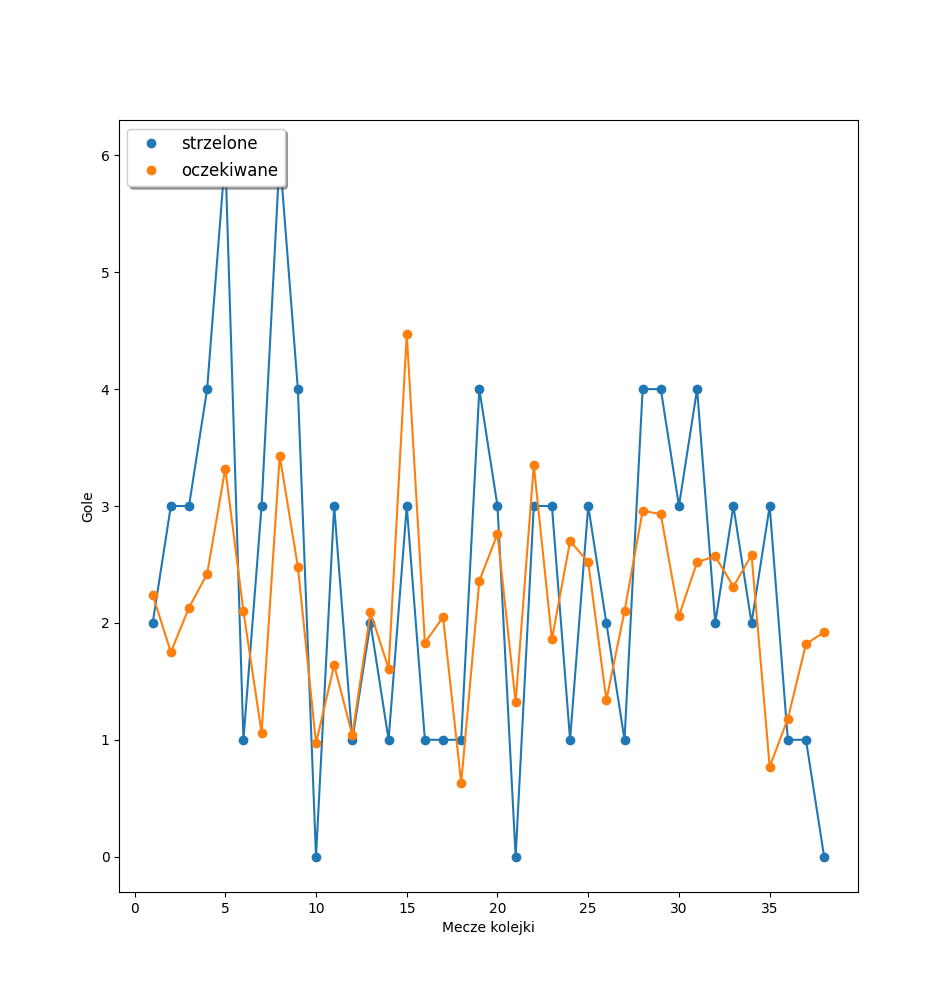
\includegraphics[width=.8\textwidth]{images/Manchester_goals.png}
    \caption{Gole Manchesteru City}
    \label{fig:enter-label}
\end{figure}
\paragraph{} Manchester ma ponadprzeciętną średnią goli, a ponadto nie zalicza spadków formy, jak można to było zauważyć u innych drużyn. Ich średnia oscyluje w oklicach 2 i wzwyż. Szczególnie wysoką formę można zauważyć w okolicach 30. kolejki.
\pagebreak
\begin{figure}[ht]
    \centering
    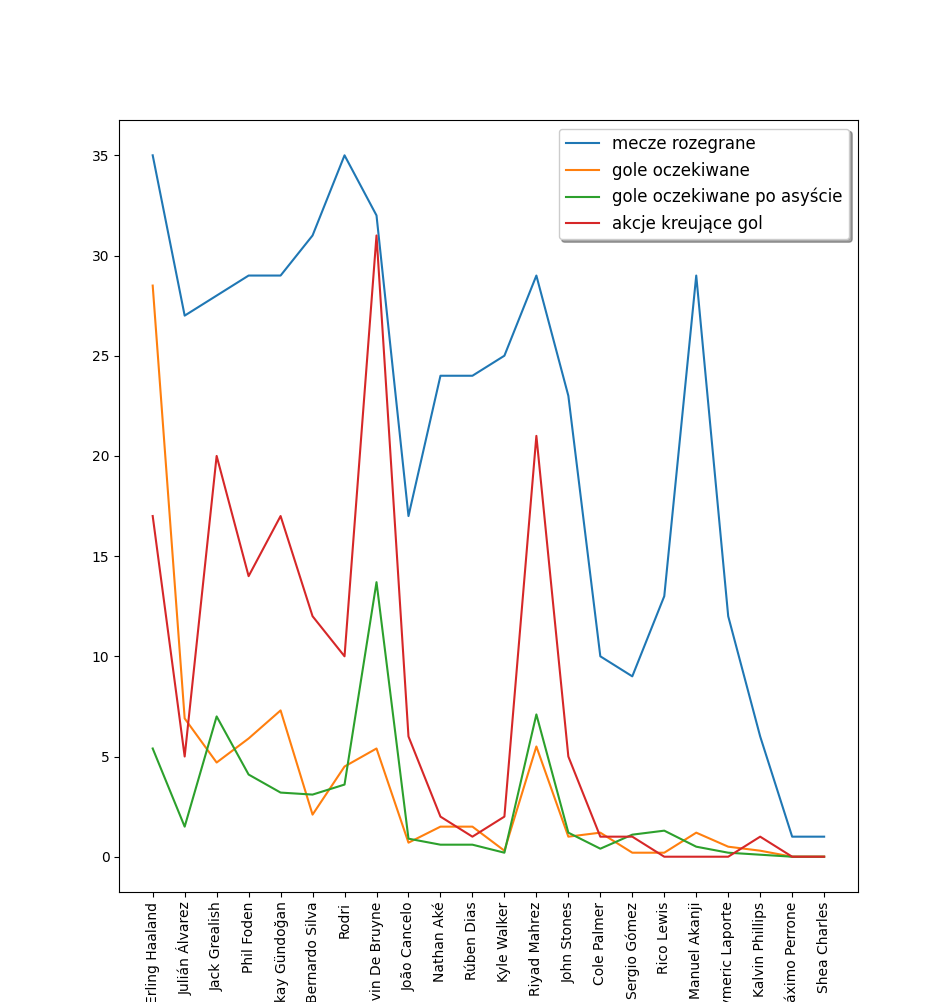
\includegraphics[width=0.8\textwidth]{images/Manchester_player_goals.png}
    \caption{Gole graczy Manchesteru City}
    \label{fig:enter-label}
\end{figure}
\paragraph{} Wykres przedstawia zaskakująco dobre statystyki. Można tutaj również wyróżnić kilku graczy, ale z pewnością cała drużyna prezentuje się nadzwyczaj solidnie. Z pewnością dwóch najbardziej odznaczających się graczy to Kevin de Bruyne, kreujący najwięcej akcji, i Erling Haaland, strzelający najwięcej goli.
\pagebreak
\begin{figure}[ht]
    \centering
    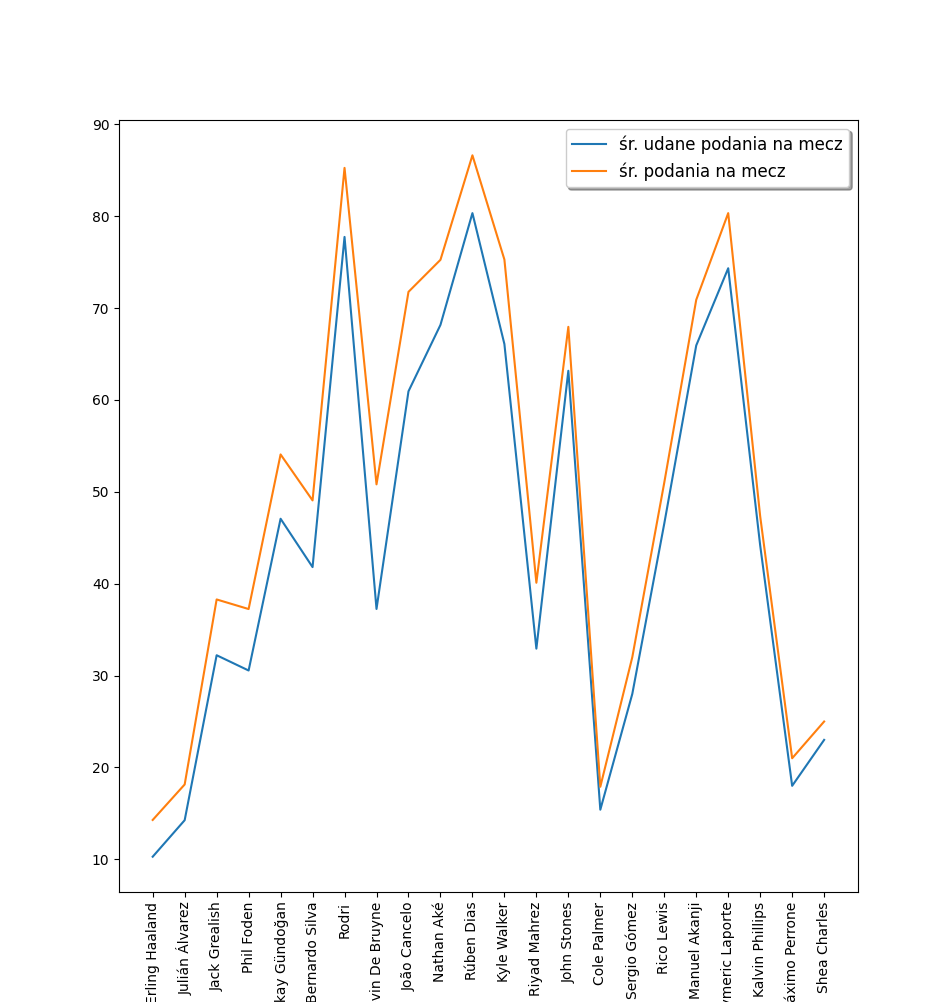
\includegraphics[width=0.8\textwidth]{images/Manchester_passes.png}
    \caption{Podania graczy Manchesteru City}
    \label{fig:enter-label}
\end{figure}
\paragraph{} Podania zawodników Manchesteru City również prezentują się nadzwyczaj dobrze. Ich ilość jest nieporównywalnie większa od innych analizowanych klubów oraz dokładność jest również na wysokim poziomie.
\pagebreak

\subsection{Rozgrywki UCL}
\paragraph{} Niestety Milan i Inter w ostatnich latach bardzo słabo wypadały w lidze mistrzów. W ciągu ostatnich 5 lat tylko Interowi raz udało się wejść do fazy pucharowej, odpadając w 1/8 finału. Tym samym oba kluby dostarczają za mało informacji do analizy. Tylko Manchester City i Real Madrid prezentowały wyniki, które można przeanalizować.
\par Dla obywdu drużyn można zauważyć trend. Naturalnie zwiększa się liczba podań, spada liczba goli oraz akcji kreujących gole ze względu na trudność rozgrywek. Pomimo tego dalej są gracze wybitni na tle reszty zespołu, przykładowo Vinicius i Modric z Realu oraz Kevin de Bruyne i Phil Foden z Manchesteru. Niemniej jednak dalej można zauważyć o wiele lepsze statystyki Manchesteru jako całego zespołu, czy pojedynczych jednostek tworzących zespół.
\pagebreak

\subsubsection{Real Madrid}
\begin{figure}[ht]
    \centering
    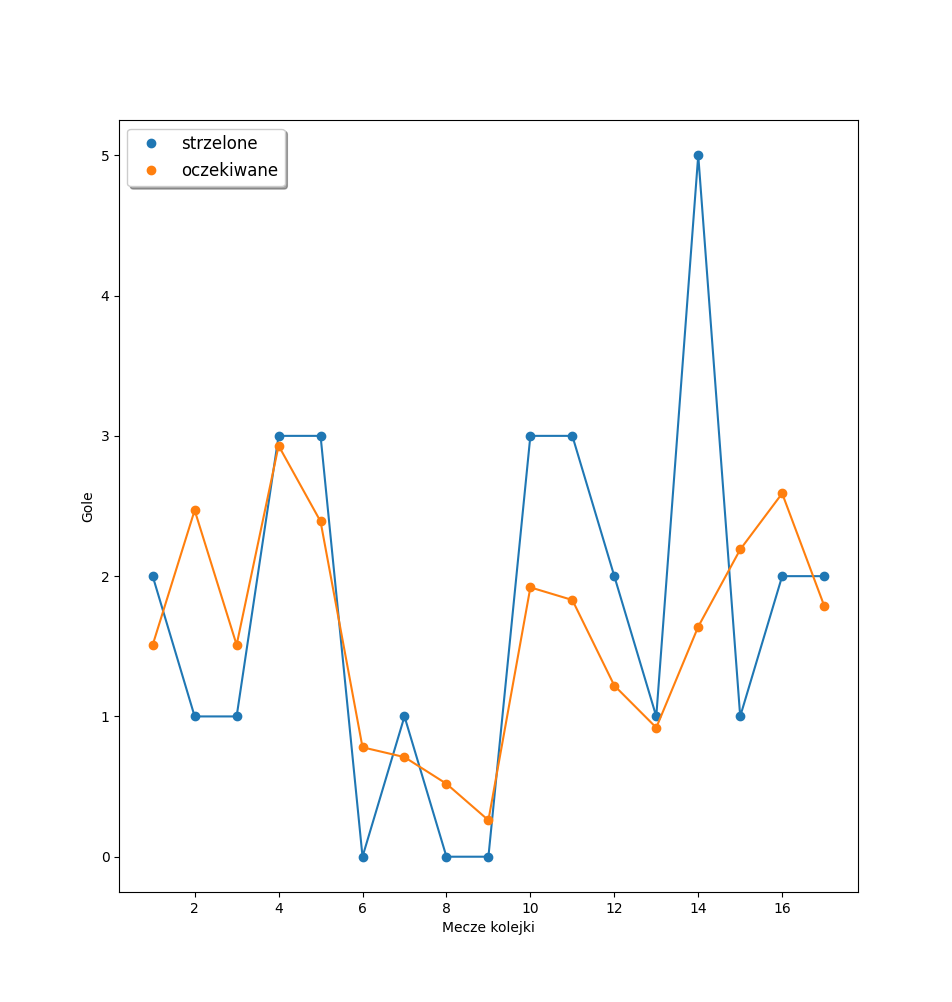
\includegraphics[width=.8\textwidth]{images/UCL_Real_goals.png}
    \caption{Gole Realu Madrid}
    \label{fig:enter-label}
\end{figure}
\pagebreak
\begin{figure}[ht]
    \centering
    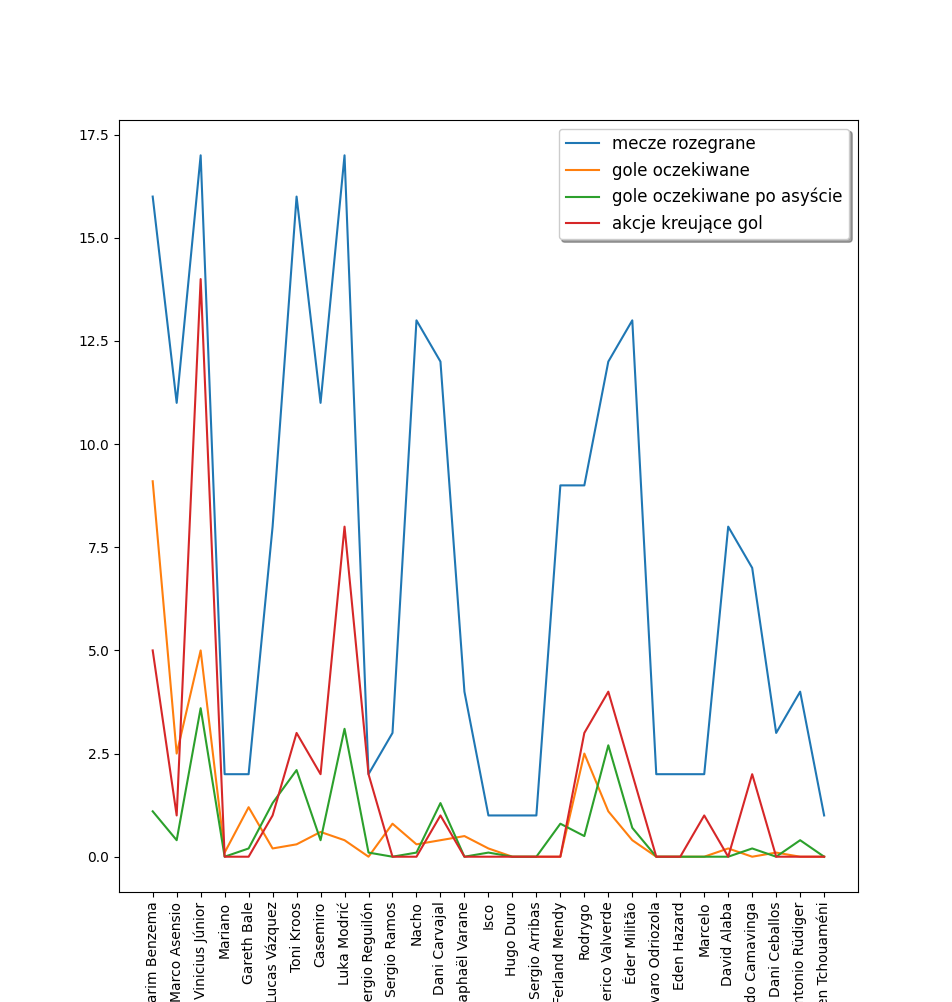
\includegraphics[width=0.8\textwidth]{images/UCL_Real_player_goals.png}
    \caption{Gole graczy Realu Madrid}
    \label{fig:enter-label}
\end{figure}
\pagebreak
\begin{figure}[ht]
    \centering
    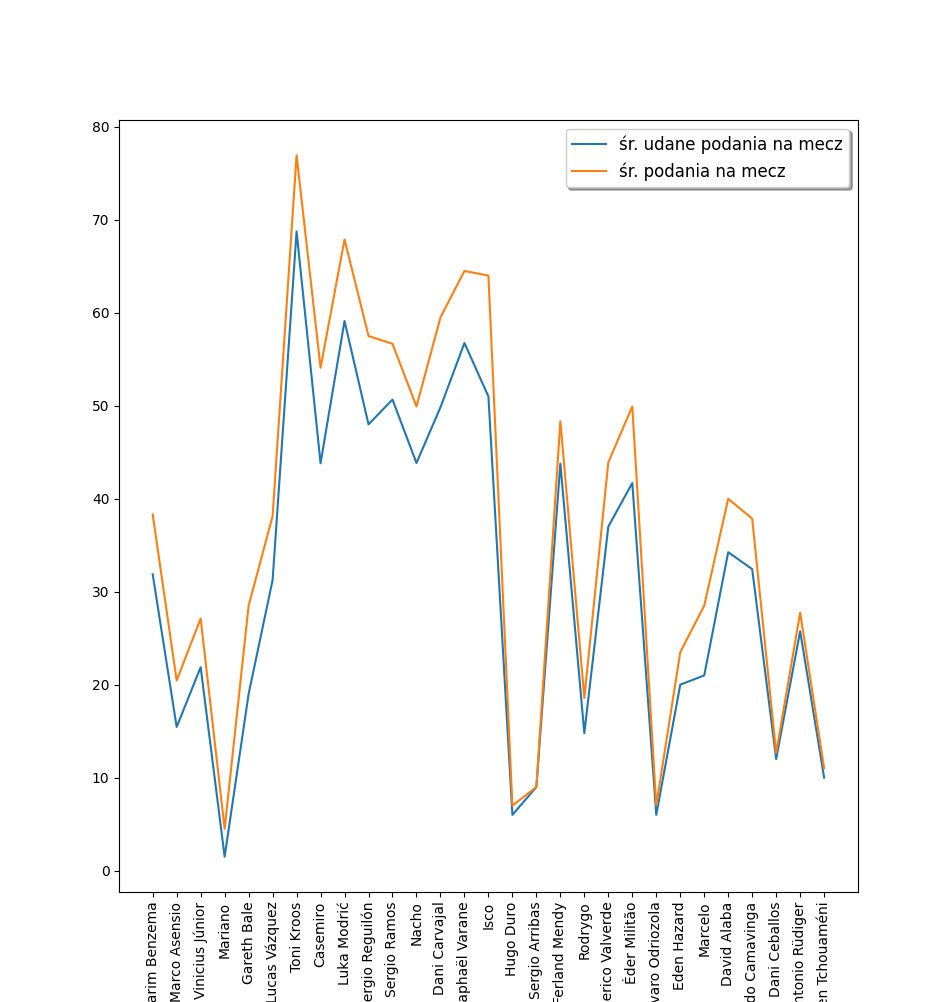
\includegraphics[width=0.8\textwidth]{images/UCL_Real_passes.png}
    \caption{Podania graczy Realu Madrid}
    \label{fig:enter-label}
\end{figure}
\pagebreak

\subsubsection{Manchester City}
\begin{figure}[ht]
    \centering
    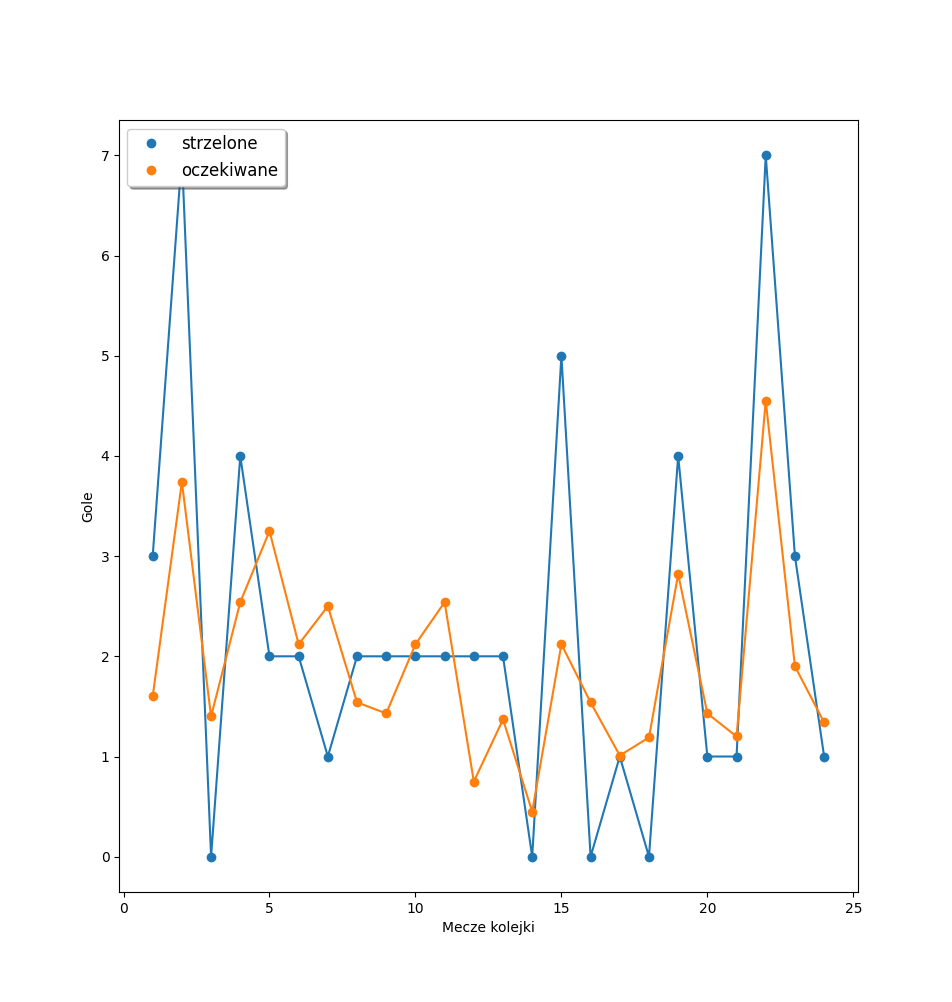
\includegraphics[width=.8\textwidth]{images/UCL_Manchester_goals.png}
    \caption{Gole Manchesteru City}
    \label{fig:enter-label}
\end{figure}
\pagebreak
\begin{figure}[ht]
    \centering
    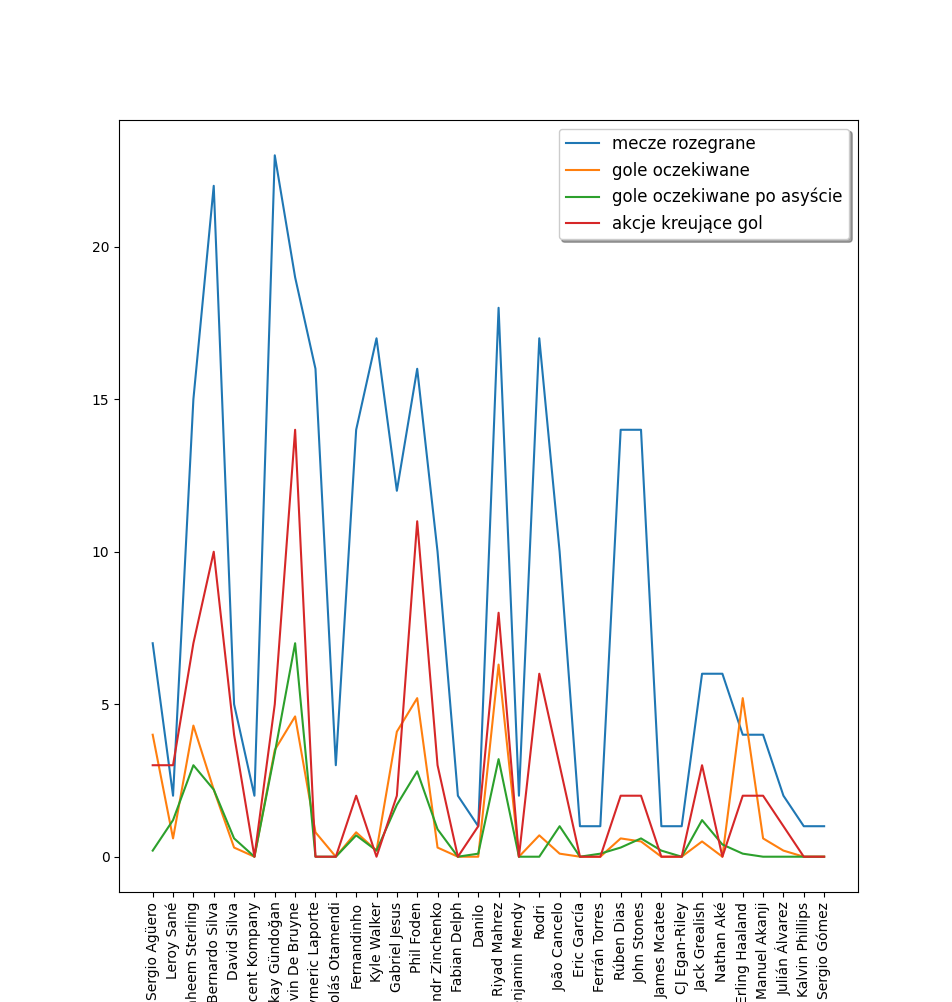
\includegraphics[width=0.8\textwidth]{images/UCL_Manchester_player_goals.png}
    \caption{Gole graczy Manchesteru City}
    \label{fig:enter-label}
\end{figure}
\pagebreak
\begin{figure}[ht]
    \centering
    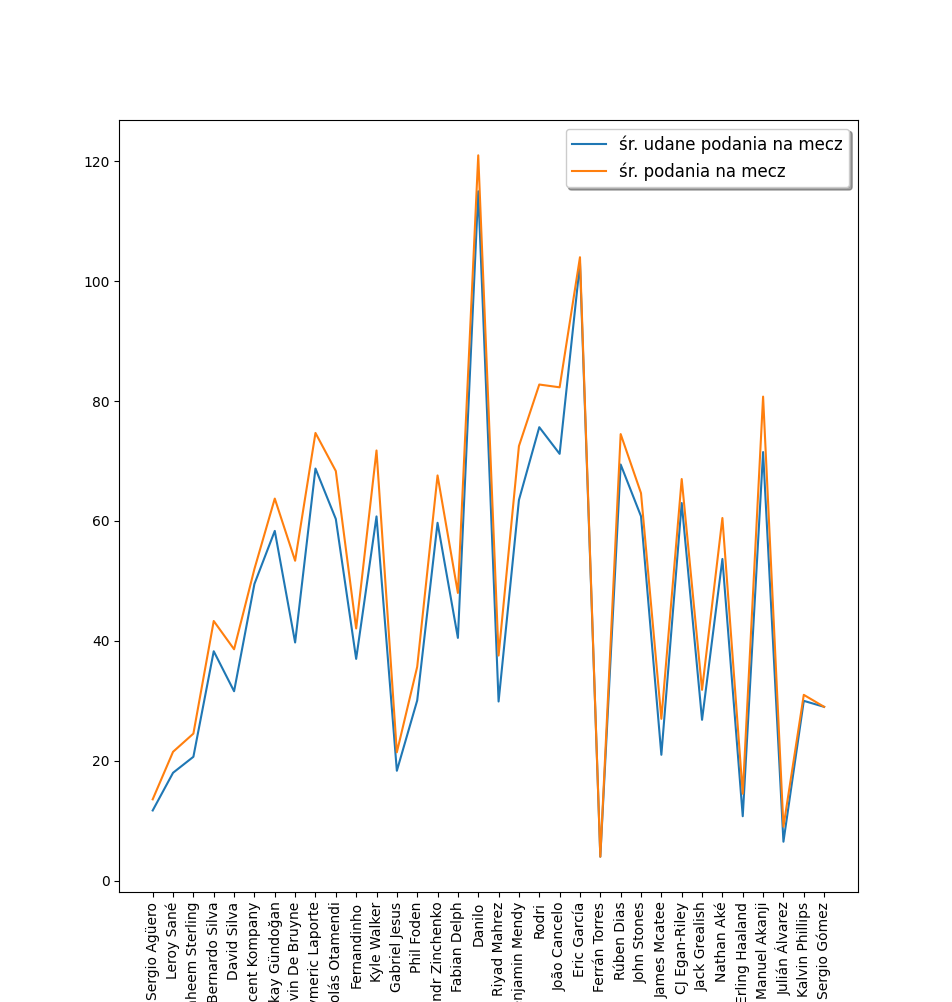
\includegraphics[width=0.8\textwidth]{images/UCL_Manchester_passes.png}
    \caption{Podania graczy Manchesteru City}
    \label{fig:enter-label}
\end{figure}
\pagebreak


\section{Modelowanie danych}
\subsection{Problem}
\paragraph{} Podane powyżej dane pozwalają zobrazować formę danych drużyn. Jednak najistotniejsze według wielu analityków jest przekształcanie okazji na bramki. Tym samym dla rozwiązywanego problemu kluczowa jest klasyfikacja zawodników obu drużyn w stosunku akcji kreujących bramki do akcji kreujących strzał.
\subsubsection{Objaśnienie}
\paragraph{} W celu zobrazowania przewagi drużyny posłużę się SVM (Support Vector Machines) służącymi między innymi do klasyfikacji. Metoda pozwala w przystępny sposób na odczytanie z wykresu żądanych informacji. W tym przypadku ma pokazywać, że klaster danej drużyny znajduje się w większości w strefie większej skuteczności względem drużyny przeciwnej. Tym samym dowodząc, że ten zespół ma większe szanse na wygraną.
\par SVM polega na wyznaczeniu płaszczyzny znajdującej się w jak największej odległości od punktów treningowych jakiejkolwiek klasy. Odległość, zwaną marginesem, od płaszczyzny do punktów SVM maksymalizuje przy pewnych założeniach.
Przykładowo parametr C umożliwia regulację pewnego dopuszczalnego dystansu, w którym się mogą znaleźć punkty treningowe. Z kolei gamma określa jądro, które udostępnia funkcję mierzącą podobienśtwo między danym punktem treningowym i innymi.
\pagebreak
\subsection{Real Madrid - Manchester City}
\begin{figure}[ht]
    \centering
    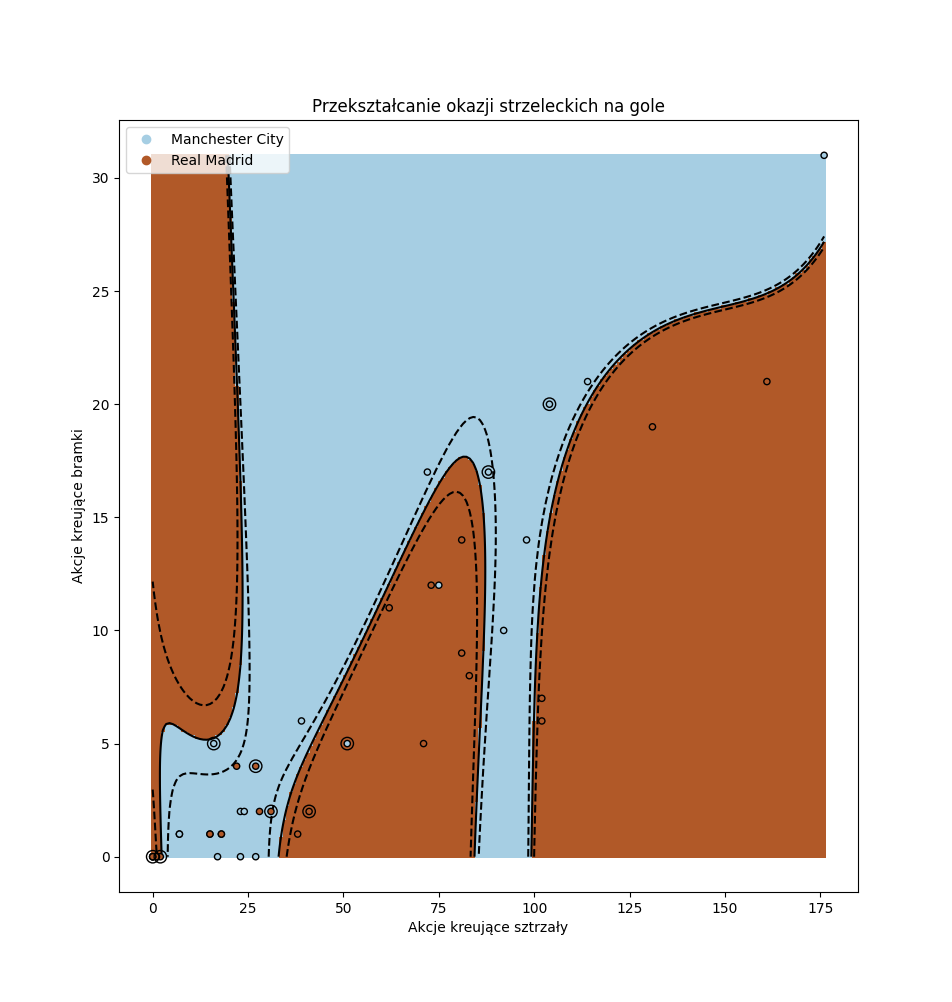
\includegraphics[width=0.8\textwidth]{images/06707506ManReal.png}
    \caption{Klasyfikacja - Real Madrid vs Manchester City}
    \label{fig:enter-label}
\end{figure}
\paragraph{} Dla powyższego wykresu: accuracy=67\%, precision=75\%, recall=60\%.
\begin{figure}[ht]
    \centering
    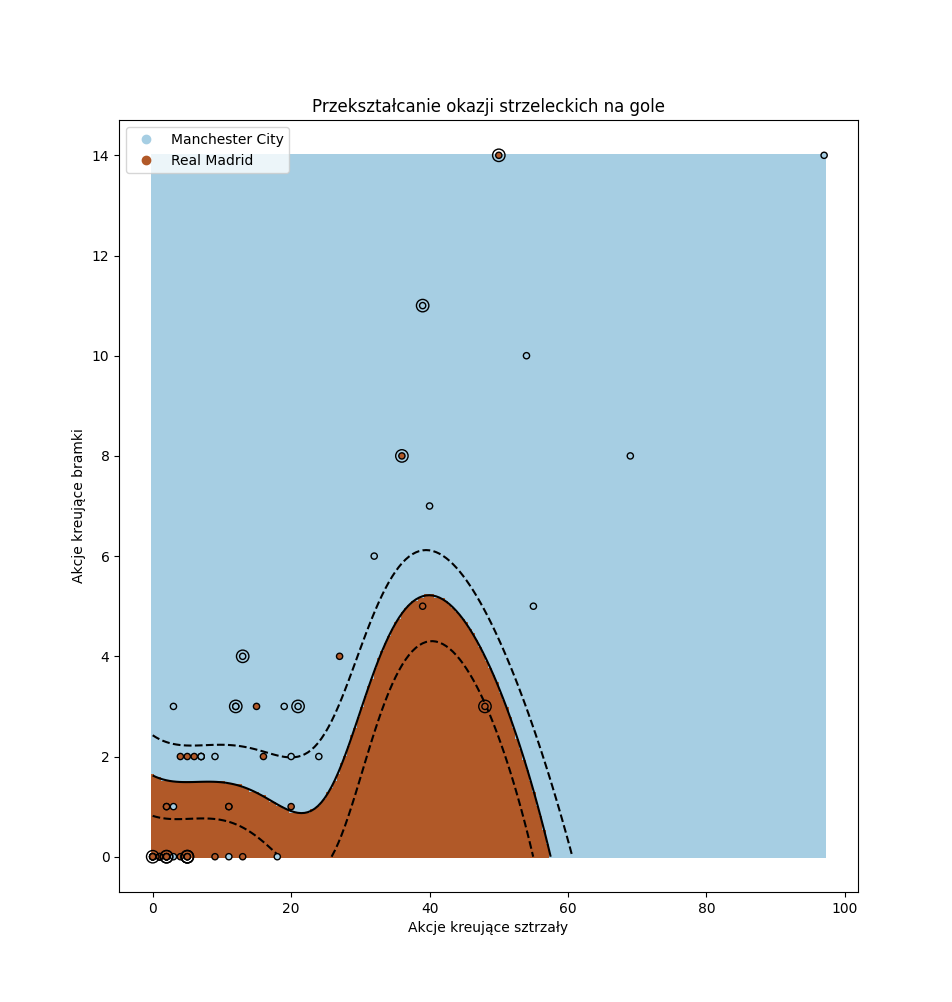
\includegraphics[width=0.8\textwidth]{images/062057067ManRealUCL.png}
    \caption{Klasyfikacja UCL - Real Madrid vs Manchester City}
    \label{fig:enter-label}
\end{figure}
\pagebreak
\paragraph{} Dla powyższego wykresu: accuracy=62\%, precision=57\%, recall=67\%.
\paragraph{} Jak można zauważyć dla dwóch powyższych wykresów Manchester zdecydowanie dominuje skutecznością nad Realem. Gracze Manchesteru zwłaszcza w rozgrywkach UCL mają więcej akcji kreujących strzały oraz większe ich przekształcanie na strzały kreujące bramki. Co jednak najważniejsze w obu przypadkach da się zauważyć gracza z niesamowitą formą (skrajny prawy górny róg). Jest to Kevin de Bruyne, który jest niewątpliwie ogromnym atutem Manchesteru.
\pagebreak
\subsection{AC Milan - Internazionale Mediolan}
\begin{figure}[ht]
    \centering
    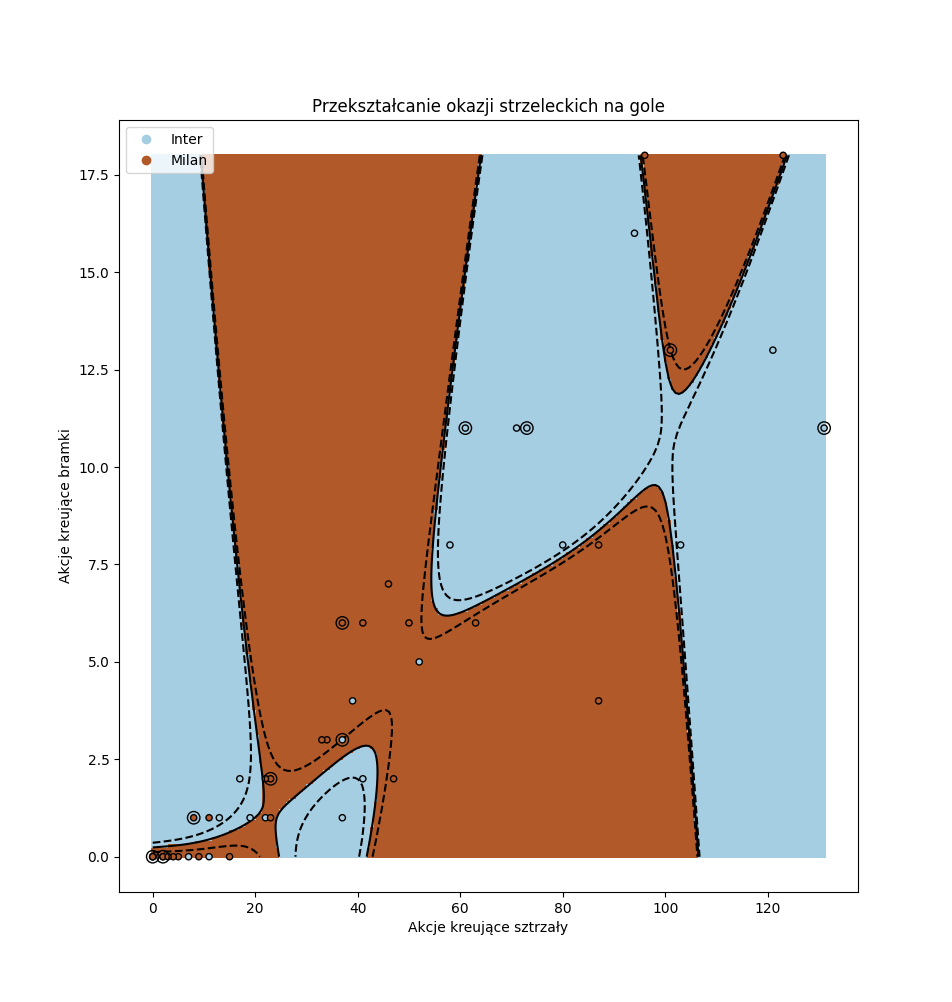
\includegraphics[width=0.8\textwidth]{images/0706708MilanInter.png}
    \caption{Klasyfikacja - AC Milan vs Internazionale Mediolan}
    \label{fig:enter-label}
\end{figure}
\paragraph{} Dla powyższego wykresu: accuracy=70\%, precision=67\%, recall=80\%.
\paragraph{} Sytuacja odnośnie dwóch mediolańskich drużyn nie jest już taka oczywista. Zawodnicy Interu z całą pewnością prezentują bardziej solidną formą. Nie da jednak nie zauważyć, że Milan posiada 3 utalentowanych graczy (Diaz, Tonali, Leao), którzy mogliby odwrócić bieg spotkania.
\pagebreak
\subsection{Finał}
\begin{figure}[ht]
    \centering
    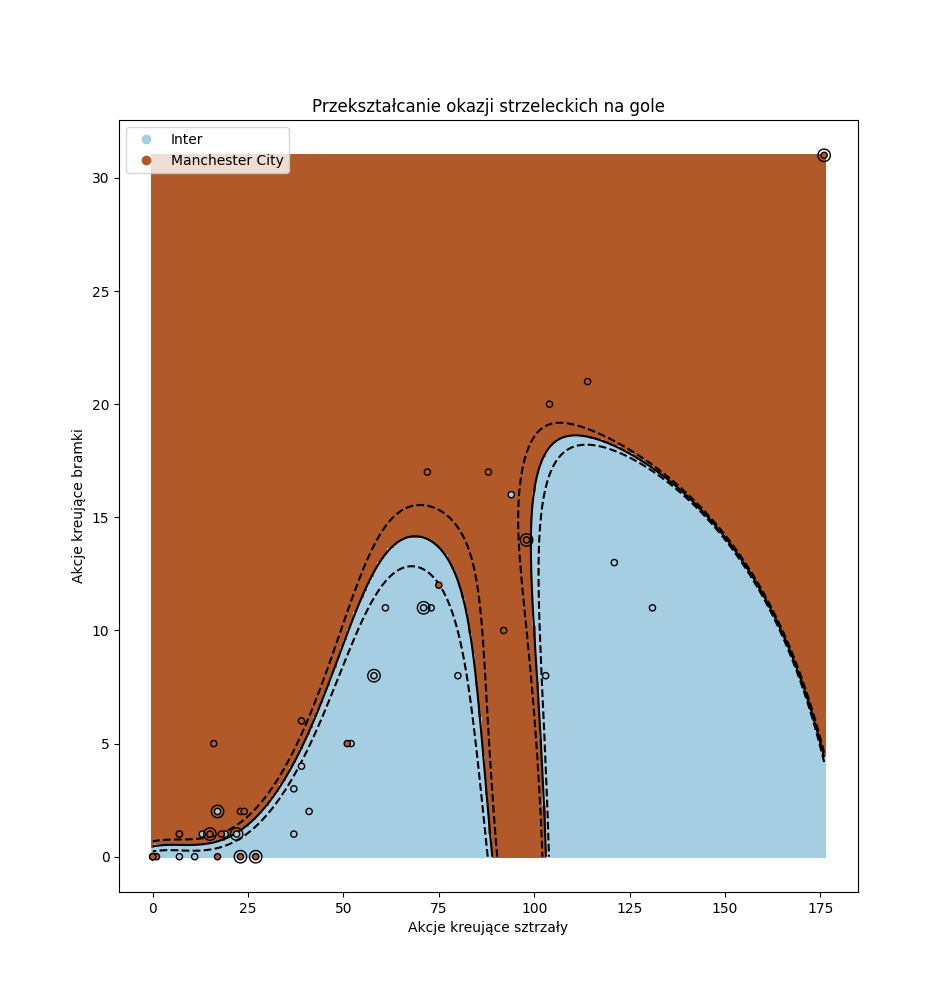
\includegraphics[width=0.8\textwidth]{images/06707506ManInter.png}
    \caption{Klasyfikacja - Manchester City vs Internazionale Mediolan}
    \label{fig:enter-label}
\end{figure}
\paragraph{} Dla powyższego wykresu: accuracy=67\%, precision=75\%, recall=60\%.
\paragraph{} Wykres prezentuje niezmienną przewagę Manchasteru nad rywalami. Chociaż można zauważyć, że gracze Interu kreują dużo akcji strzeleckich, nie potrafią ich wykorzystać. Jakość gry świadczy zdecydowanie na korzyść Manchesteru City.
\section{Wnioski}
\paragraph{} Na podstawie wstępnej analizy danych jak również wykonanego modelu obrazującego stosunek kreowania akcji bramkowych do akcji strzeleckich można z całą pewnością założyć, że zwycięzcą tegorocznej edycji UCL będzie Manchester City. Ponadto znani już finaliści, czyli Internazionale Mediolan i Manchester City, również zdają się być zasłużeni. Największe wątpliwości można wobec Interu, którego model niejednoznacznie pokazał silniejszą drużynę.
\subsection{Podsumowanie}
\paragraph{} Rozwiązując problem wyłonienia najlepszej drużyny ciężko jest uzasadnić swoją decyzję, ponieważ na wygraną składa się bardzo wiele czynników. Niemniej w sporcie często tylko jedno ma znaczenie - wynik. Uznałem tym samym, że w piłce nożnej nic innego, jak tworzenie akcji strzeleckich oraz ich skuteczność może zobrazować potęgę drużyny. \par Ponadto rzeczywisty wynik meczu może nie odwzorowywać statystyk i prognoz. Nie da się jednoznacznie go stwierdzić. Można udostępnić najwyżej wykresy i zestawienia do własnej analizy odbiorcy dodając również coś od siebie.
\subsection{Prawdziwy wynik fianłu}
\paragraph{} Na chwilę pisania tego raportu wynik finału UCL 2023 jest już znany. Wygrał Manchester City, co odpowiada przewidywaniu na podstawie wykorzystanego modelu.
\subsection{Komentarze i ulepszenia}
\paragraph{} Obrany model SVM nie cechował się zbyt dużą dokładnością nawet przy zmianie parametrów, np. wykorzystując inne jądro. Z pewnością modele lepiej by sobie poradziły, jeżeli nie uwzględnić w analizowanych danych graczy tworzących mnież niż X akcji, którzy są zazwyczaj obrońcami i nie mają zbyt dużego wkładu ofensywnego. Przykładową wartością X na podstawie modeli można przyjąć 30. \par Ponadto zmienna C odpowiadająca za regularyzację dopasowania krzywej musiała przyjmować duże wartości ze względu na duże zagęszczenie wartości graczy innych drużyn. Natomiast zmianny gammy, czyli wpływ jednego treningowego obiektu, powodowała bardzo nieprzewidywalne zmiany, tym samym była ciężka do własnoręcznego ustawienia.

\bibliographystyle{plain}
\bibliography{mybib}

\end{document}